\section{Metodologías para el desarrollo de Ontologías}

En este apartado se dará un resumen de las metodologías más utilizadas para la creación de una ontología; Ontology Development 101, OntoKnowledge , Methontology, y NeOn. Luego se realizará un análisis y elección según los requerimientos de este trabajo.

\subsection{Ontology Development 101}

Esta metodología describe una serie de pasos y recomendaciones a la hora de crear una ontología. 

Se describen a continuación los pasos:
\begin{description}
\item[Paso 1:] Determinar el dominio y alcance de la ontología.
\item[Paso 2:] Considerar la reutilización de ontologías.
\item[Paso 3:] Enumerar términos importantes de la ontología.
\item[Paso 4:] Definir las clases y las jerarquías de las clases.
\item[Paso 5:] Definir las propiedades de las clases.
\item[Paso 6:] Definir las características de cada clase y propiedad.
\item[Paso 7:] Crear instancias.
\end{description}

Además la guía propone algunas buenas prácticas de desarrollo de ontologías relacionadas a la definición de clases como la correcta creación de jerarquías, herencias múltiples,  cuándo crear una clase o una propiedad, cuando es una instancia o una clase, etc. También algunos delineamientos sobre las propiedades como valores por defecto, cardinalidad, etc. Por último, una serie de convenciones de nombres dentro de la ontología. La metodología no tiene en cuenta el proceso de especificación ni el mantenimiento de la ontología.

\subsection{OntoKnowledge} 

Ontoknowledge propone crear ontologías teniendo en cuenta su uso posterior en sistemas de administración de conocimiento, por tanto las ontologías creadas son dependientes de la aplicación. La metodología incluye la identificación de metas a ser logradas a través de herramientas de control basadas en los escenarios de usos.

El proceso que propone la metodología se puede resumir en los siguientes pasos:

\textbf{Estudio de Factibilidad.} Esta debe ser aplicada a toda la aplicación y debe llevarse a cabo antes del desarrollo de la ontología. Aquí se identifica el problema y las áreas de oportunidades, se selecciona la mejor área de enfoque para la solución.

\textbf{Patada Inicial.} El resultado de este proceso es el Documento de Especificación de Requerimientos de la Ontología (ORSD). Se describen las metas y el dominio de la ontología, líneas de diseño (convenciones de nombres), lista de recursos disponibles (libros, revistas, documentación, etc), potenciales usuarios y casos de uso, así como las aplicaciones que utilizarán la ontología. Para esto se propone crear una lista de preguntas de competencia las cuales debe satisfacer la ontología creada. Los conceptos y relaciones más importantes son identificados en un nivel informal. También se debe de buscar ontologías para su potencial reuso, la metodología no provee un delineamiento para identificar dichas ontologías.

\textbf{Refinamiento.} Aquí se construye una ontología sólida orientada a la aplicación acorde al proceso de especificación. Este proceso se divide en dos actividades:

\begin{description}
\item[Actividad 1:] Extracción del conocimiento del los expertos del dominio. Los axiomas de la ontología son definidos y modelados por los expertos del dominio. La metodología propone el uso de una representación intermedia para modelar el conocimiento.
\item[Actividad 2:] Formalización de la ontología. La ontología es implementada en un lenguaje ontológico, el lenguaje es seleccionado según los requerimientos del uso de la ontología.
\end{description}

\textbf{Evaluación.} Este paso sirve para probar la usabilidad de la ontología desarrollada dentro del entorno para la cual fue desarrollada. En este proceso se verifica que se puedan responder las preguntas de competencia y que se satisfagan los requerimientos, además se prueba la ontología en el entorno de software para el cual se desarrolló.

\textbf{Mantenimiento.} En esta etapa es importante recalcar quién es el responsable de mantener la ontología y cómo se debe hacerlo.

La metodología propone un ciclo de vida incremental y cíclico como se muestra en la Figura \ref{img:ontoknowledge}.

\begin{figure}[h!]
    \centering
    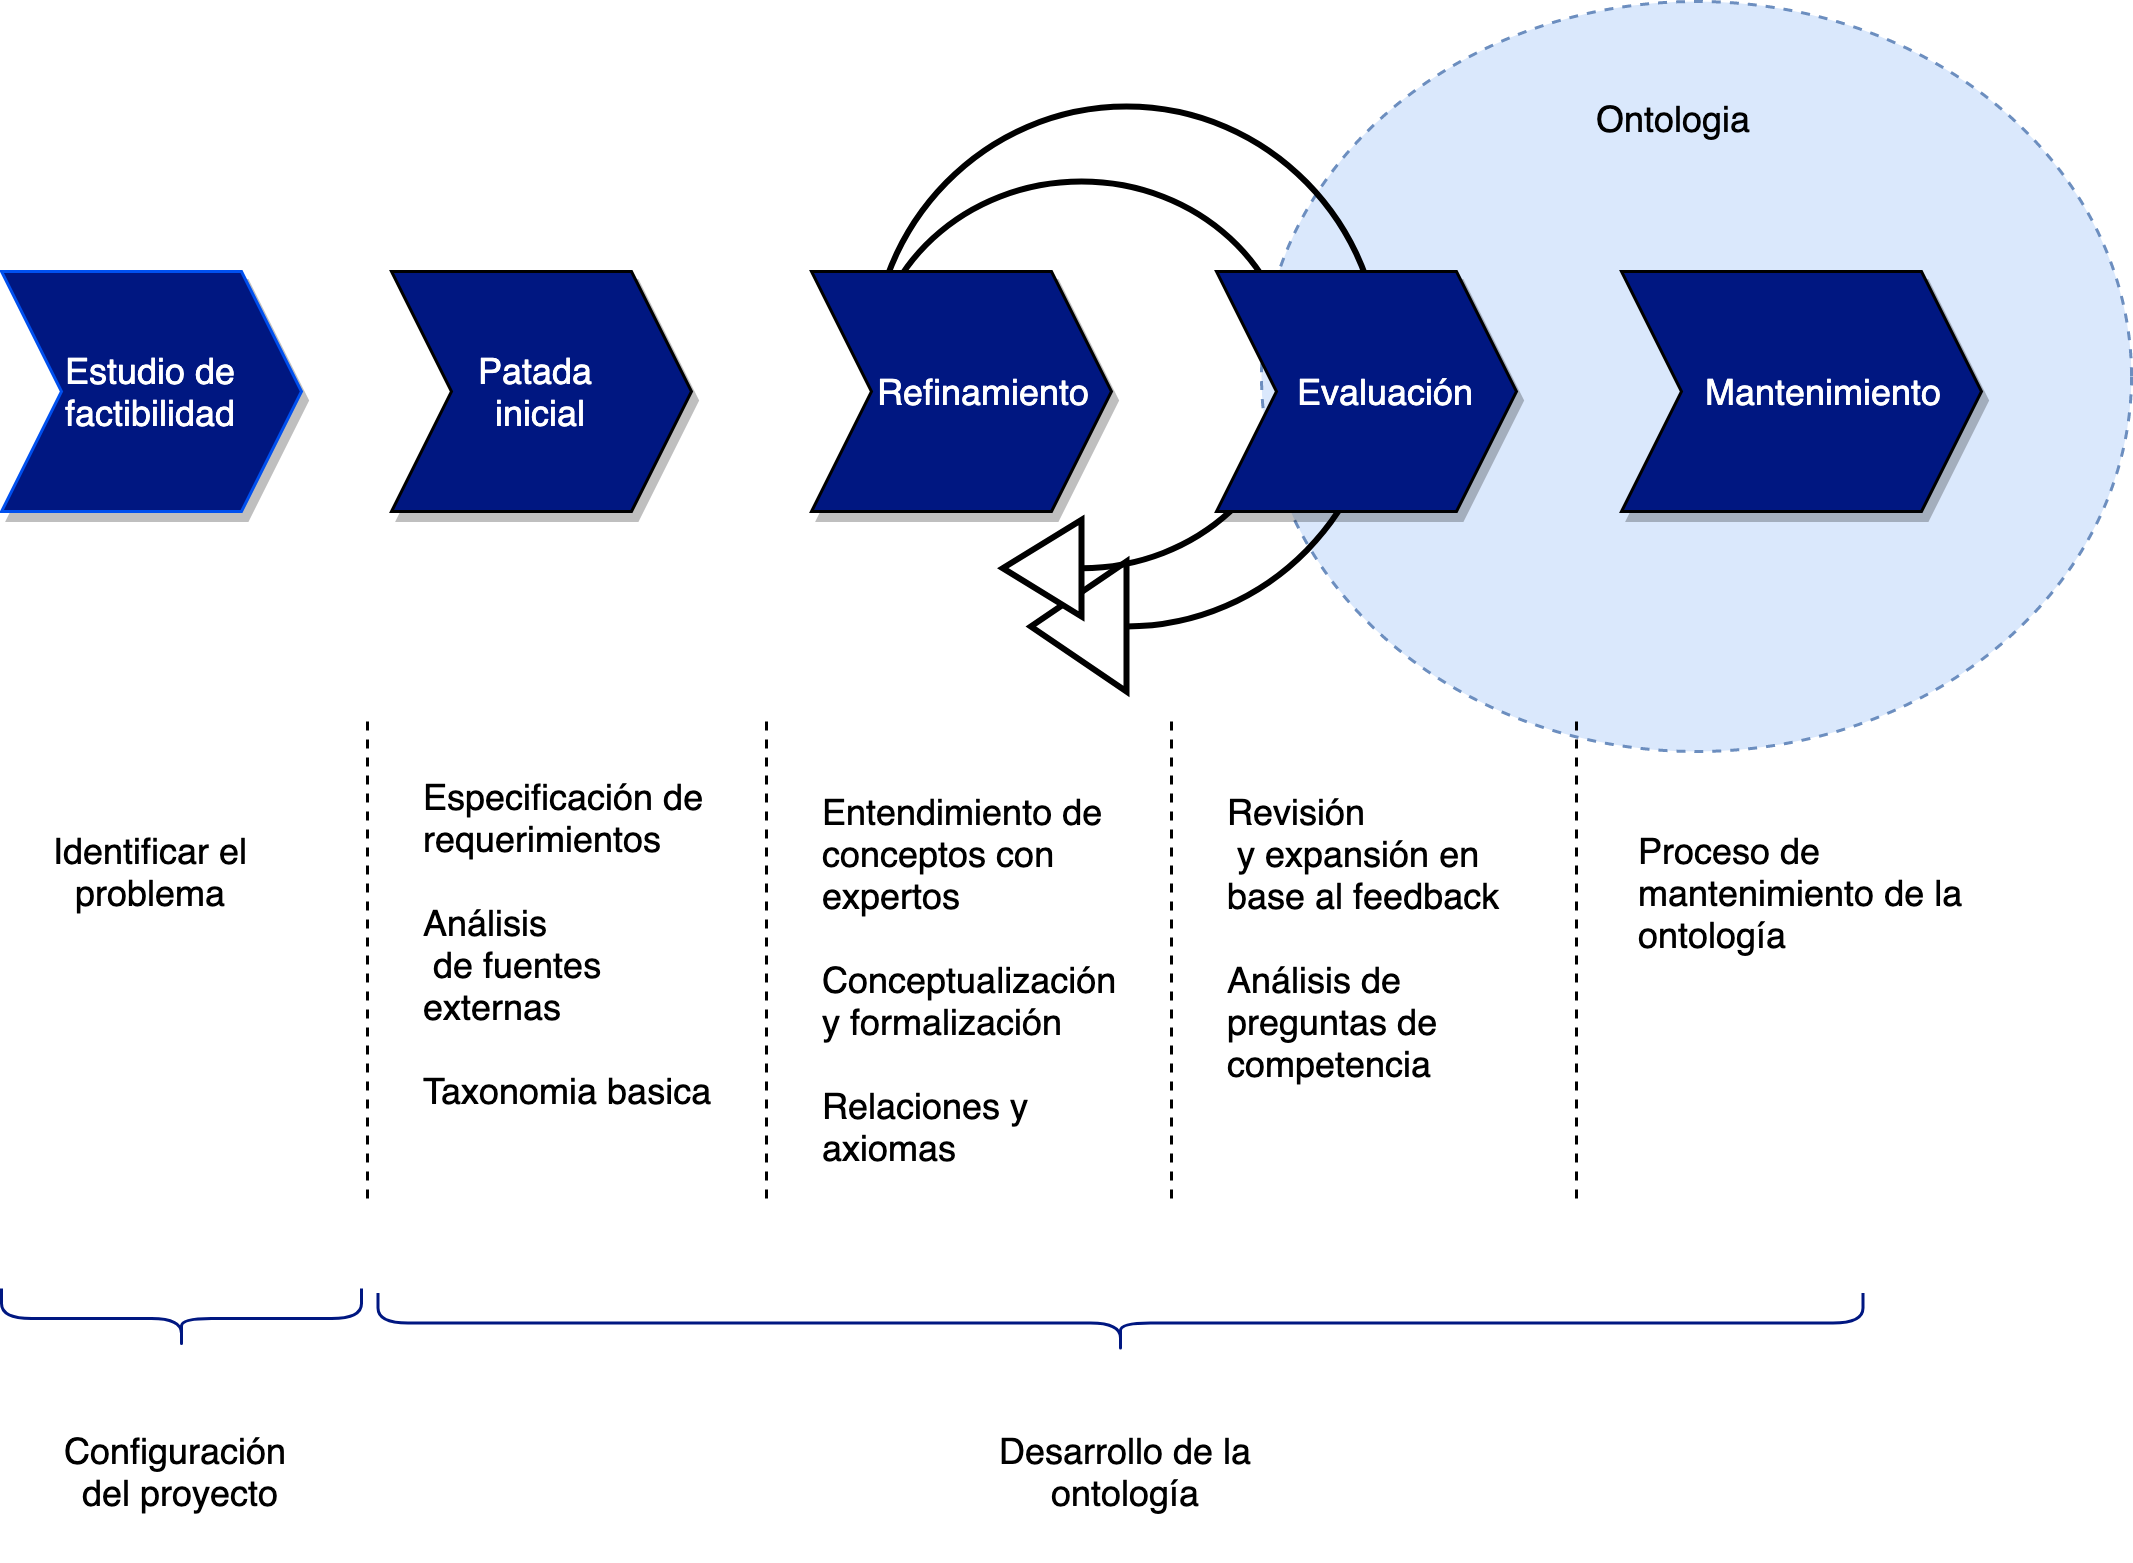
\includegraphics[width=150mm]{figuras/Diagramas-OntoKnowledgeProcess}
    \caption{Ciclo de vida de OntoKnowledge}
    \label{img:ontoknowledge}
    \end{figure}

\subsection{Methontology}

Esta metodología incluye la identificación del proceso del desarrollo de una ontología, que consiste en una serie de actividades, el ciclo de vida basado en el refinamiento de un prototipo y técnicas para llevar a cabo cada actividad durante el mantenimiento, el desarrollo y el soporte de las actividades. Todas las actividades están basadas en el proceso de desarrollo de software y las utilizadas en metodologías de ingeniería de conocimiento.

En la Figura \ref{img:methontology} se puede ver los estados de todo el ciclo de vida de la ontología.

\begin{figure}[h!]
    \centering
    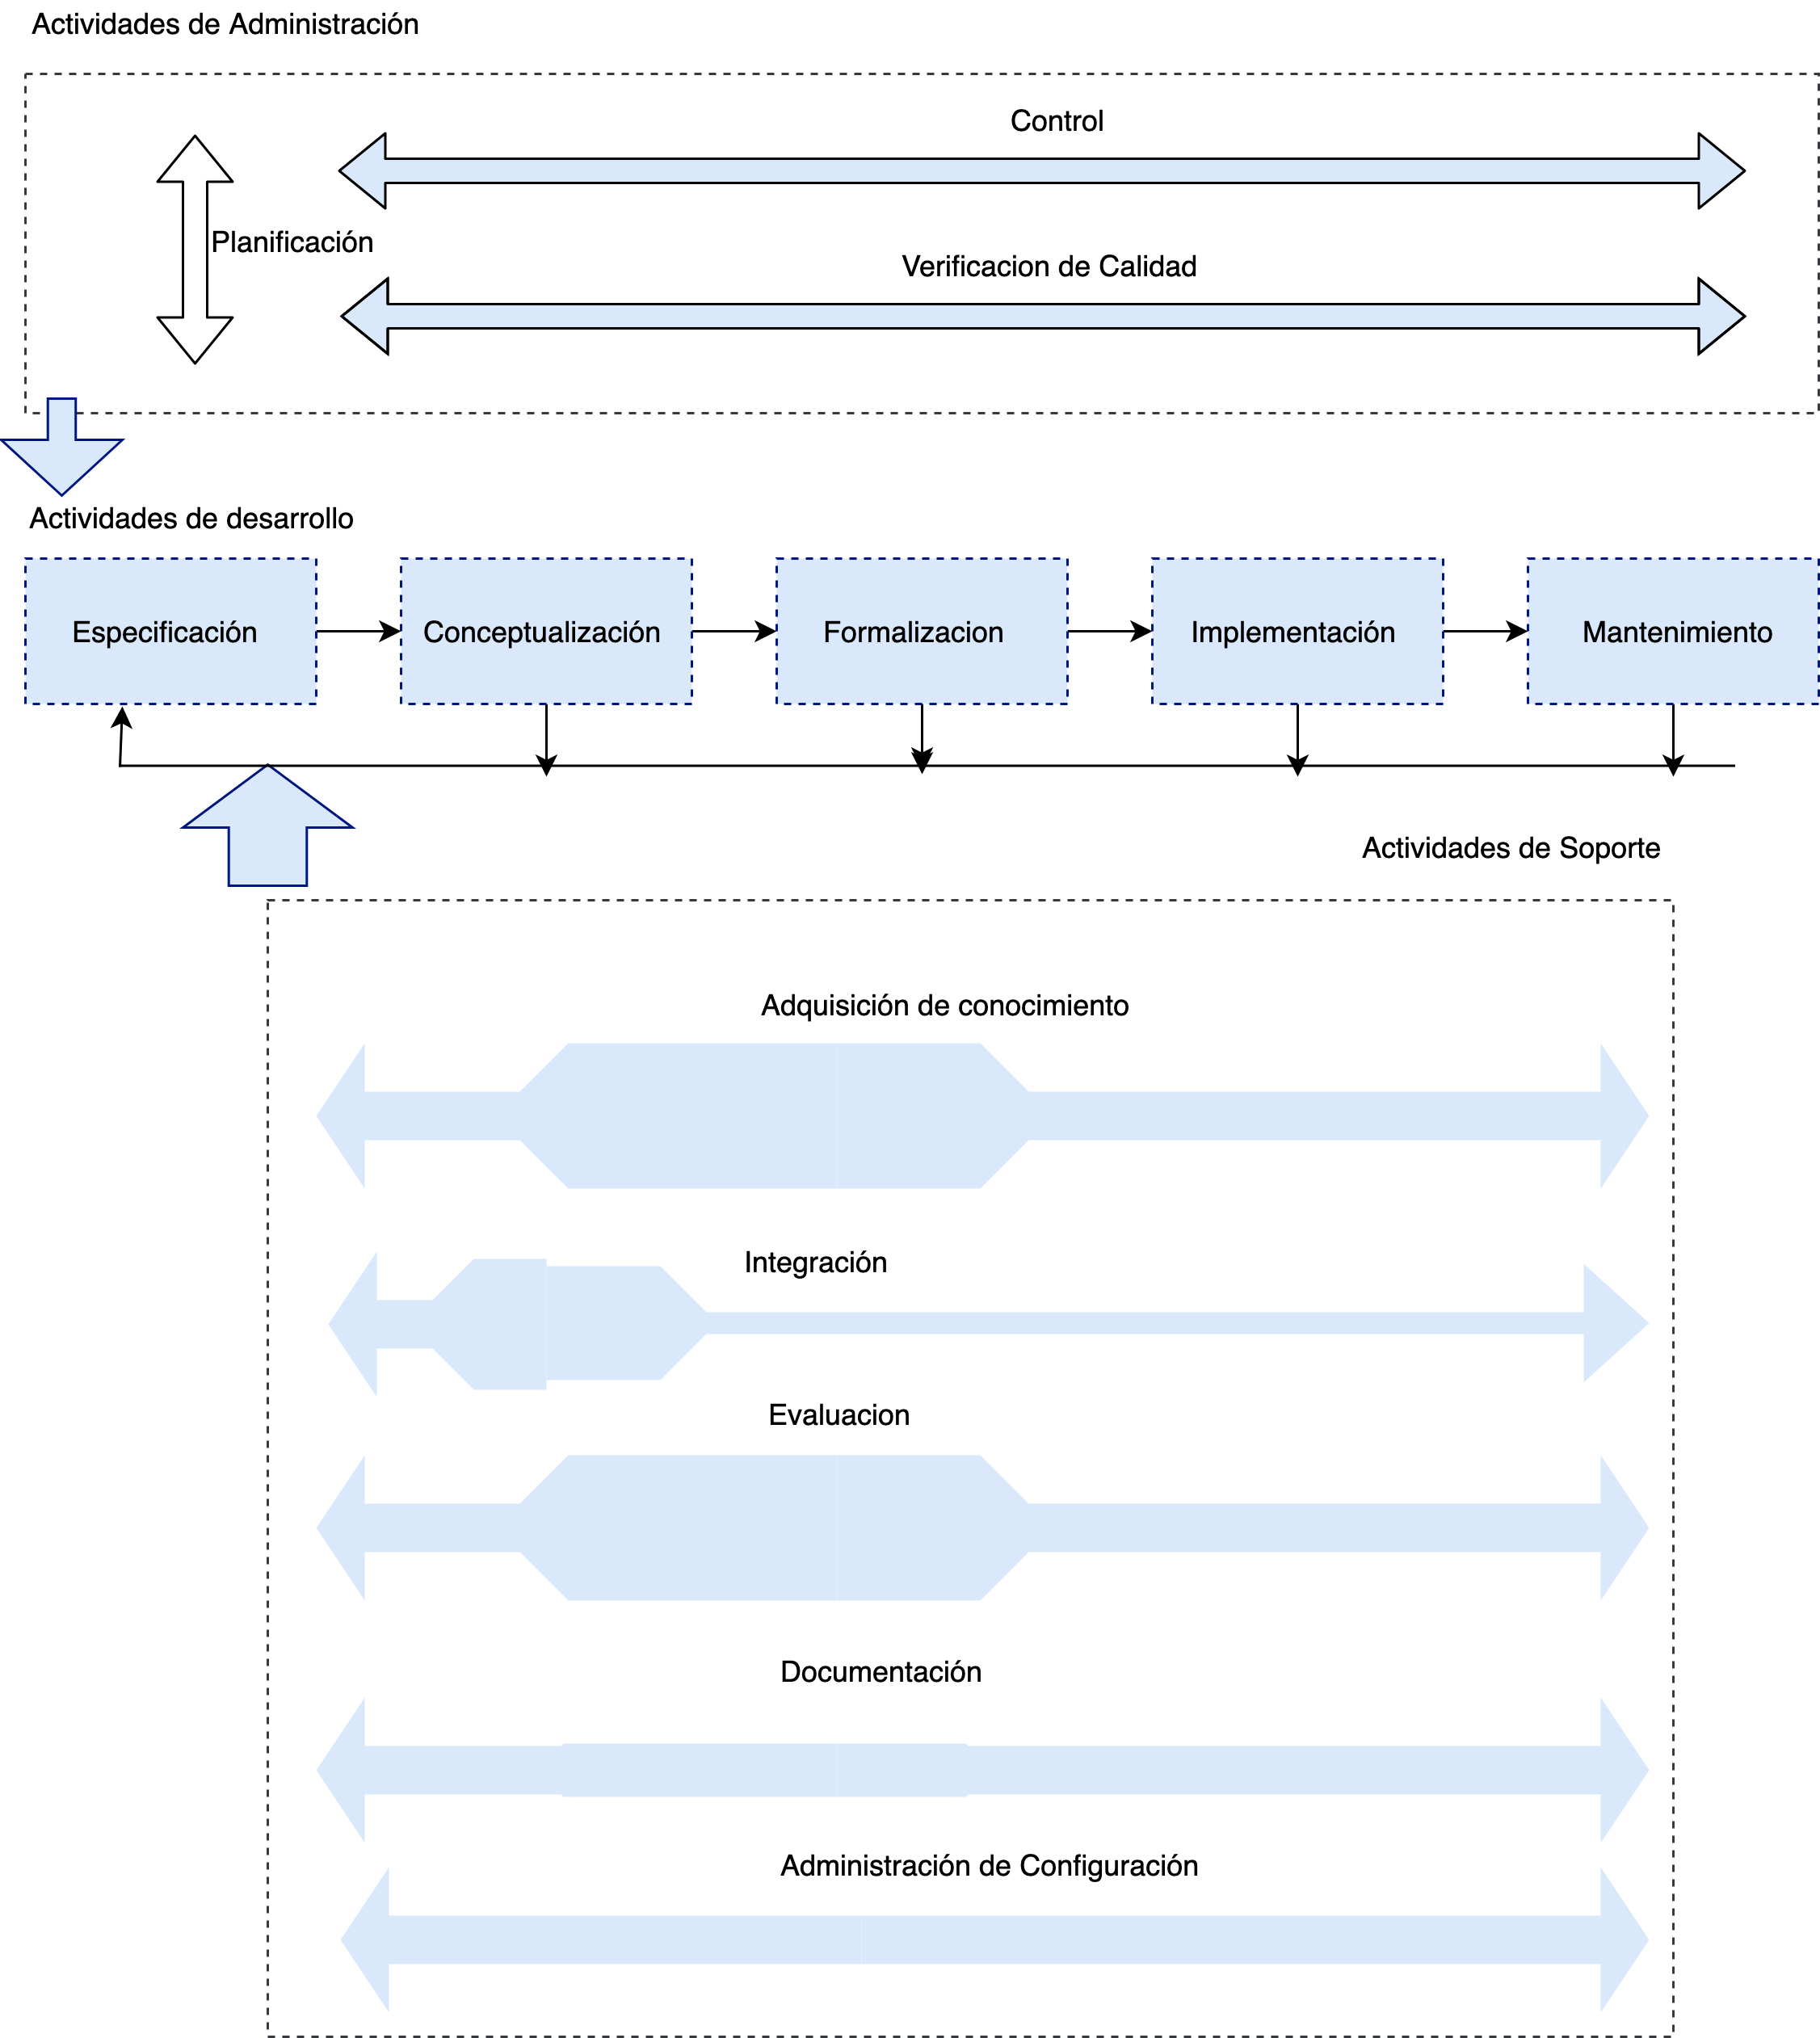
\includegraphics[width=150mm]{figuras/Diagramas-MethontologyProcess}
    \caption{Ciclo de vida de Methontology}
    \label{img:methontology}
    \end{figure}
    
    
La metodología propone un ciclo de vida basado en prototipos que permite agregar, cambiar y remover términos en cada prototipo. Para cada prototipo, se propone comenzar con la planificación para identificar las tareas, tiempos y recursos necesarios. Luego, comienza la actividad de especificación, con ella comienzan las actividades de gestión (Control y Calidad) y procesos de soporte (Adquisición de conocimiento, integración, evaluación, documentación y gestión de la configuración), todo esto ejecutado en forma paralela a las actividades de desarrollo (especificación, conceptualización, implementación y mantenimiento) durante todo el ciclo de vida de la tecnología \cite{fernandez1997methontology}.
 
A continuación se describen algunas de las principales actividades:

\begin{enumerate}
\item \textbf{Especificación:} Especificar el propósito de la ontologías, esto incluye usuarios, contexto, nivel de formalidad esperado y granularidad. El resultado de esta fase es un documento de especificación de la ontología en lenguaje natural.
\item \textbf{Adquisición} de conocimiento: Esto ocurre en paralelo a las demás fases, pero específicamente en la parte de especificación. Se consultan libros, manuales, tablas, otras ontologías y expertos para adquirir conocimientos sobre el área a modelar.
\item \textbf{Conceptualización:} Se identifican los términos según sean conceptos, instancias, relaciones o propiedades para crear un modelo conceptual del dominio.
\item \textbf{Integración:} En esta fase se considera el reuso de términos de otras ontologías para no volver a definir y ahorrar trabajo.
\item \textbf{Implementación:} La ontología es representada formalmente en un lenguaje tipo OWL o RDFS.
\item \textbf{Evaluación:} Significa hacer un juzgamiento técnico de la ontología creada, el entorno de desarrollo y la documentación de la misma. La evaluación está compuesta por la verificación y la validación.
\item \textbf{Documentación:} El cual consiste en todos los documentos producidos durante el desarrollo de la ontología que va desde el mismo código de la ontología hasta artículos científicos de la misma.
\end{enumerate}


\subsection{NeOn}
Esta metodología incluye métodos, técnicas y herramientas para llevar a cabo actividades para el proceso de desarrollo de una red ontológica. Está enfocada en la especificación de los requerimientos, la planificación y el reuso de recursos ontológicos y no-ontológicos \cite{suarez2010neon}.

La metodología presenta los siguientes componentes:
\begin{itemize}
    \item Un glosario: Identifica y define los procesos y actividades que pueden estar dentro de el desarrollo de una ontología. En la Figura \ref{img:neon actividades} se muestra la lista de procesos y actividades divididas según la fase de desarrollo.
    \item Nueve escenarios para el desarrollo de ontologías. Se identificaron nueve escenarios flexibles para el desarrollo de ontologías, donde cada escenario está compuesto de diferentes procesos y actividades. En la Figura \ref{img:neon ciclo de vida} se distinguen las relaciones entre las actividades y los escenarios donde las fechas dirigidas con círculos numerados asociados representan los diferentes escenarios. 
    \item Una serie de guías metodológicas para procesos y actividades como el reuso de recursos ontológicos y no-ontológicos, la especificación de los requerimientos, la planificación, etc. Los procesos y actividades están representados en la Figura \ref{img:neon ciclo de vida} con cajas y círculos de color.
\end{itemize}

A continuación se presenta el glosario de términos:
\begin{figure}[h!]
    \centering
    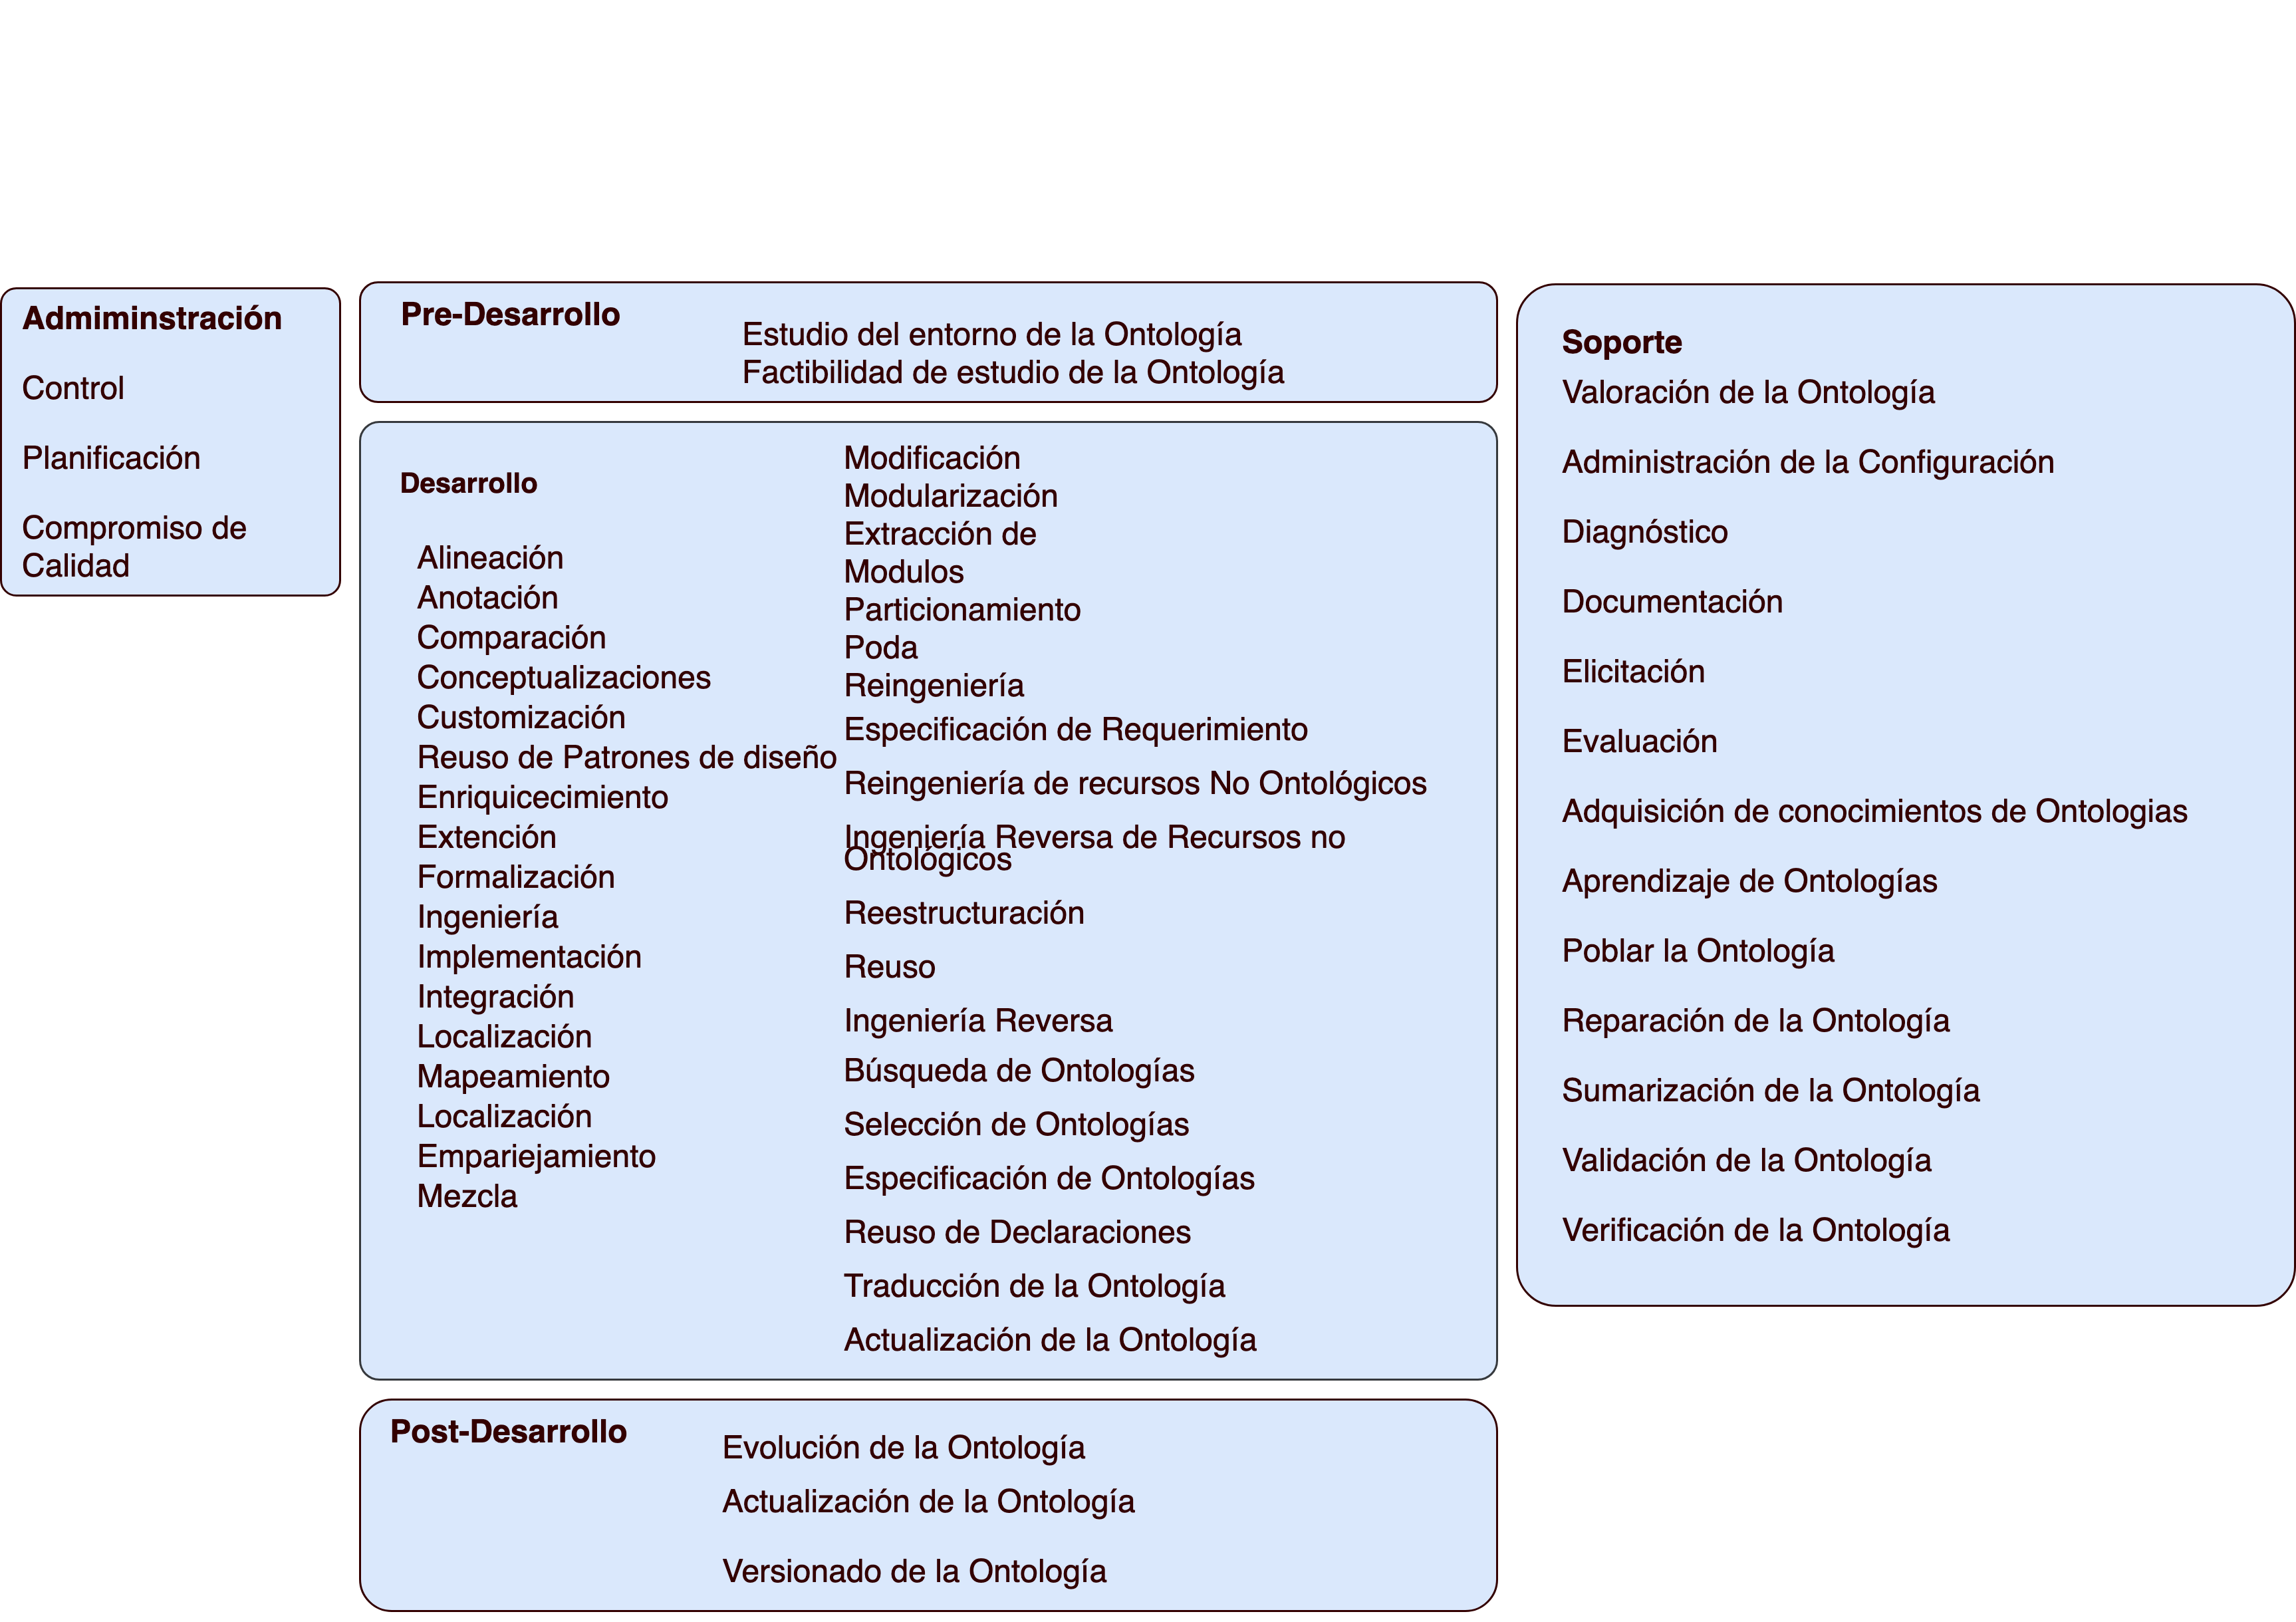
\includegraphics[width=150mm]{figuras/Diagramas-NeonActivities}
    \caption{Actividades de NeOn}
    \label{img:neon actividades}
    \end{figure}


A continuación se presentan los nueve escenarios que propone NeOn.

\begin{description}
    \item[Escenario 1] El escenario va desde la especificación hasta la implementación. La ontología es desarrollada desde el principio, esto significa sin utilizar ninguna base de conocimiento ya construida.
    \item[Escenario 2] Reuso y Reingeniería de recursos no-ontológicos. Este escenario cubre el caso donde los desarrolladores analizan recursos no-ontológicos, y deciden según los requerimientos, qué recurso no-ontológico se puede reutilizar para construir esta ontología. Este escenario también realiza una reingeniería del recurso seleccionado.
    \item[Escenario 3] Reuso de recursos ontológicos. En este escenario los desarrolladores reusan recursos ontológicos, esto se puede hacer de tres maneras: reuso total, reuso de módulos y/o reuso de sentencias.
    \item[Escenario 4] Reuso y reingeniería de recursos ontológicos.Aquí, los desarrolladores hacen tanto un reuso como una reingeniería de los recursos ontológicos.
    \item[Escenario 5] Reuso y unión de recursos ontológicos. Este escenario es propicio cuando se eligen muchas ontologías del mismo dominio de conocimiento para reutilizar y se quiere crear una nueva ontología a partir de ellas.
    \item[Escenario 6] Reuso, unión y reingeniería de recursos ontológicos. Similar al escenario 5, aquí los desarrolladores realizan un proceso de reingeniería antes de unir los recursos reutilizados.
    \item[Escenario 7] Reusos de patrones de diseño de ontologías (ODP). En este escenario se utilizan repositorios de ODP para reutilizarlos.
    \item[Escenario 8] Reestructuración de recursos ontológicos. Se reestructuran recursos ontológicos, esto significa modularizar, recortar, extender y/o especializar el recurso ontológico para integrarla a la ontología construida.
    \item[Escenario 9] Localización de un recurso ontológico. En este escenario se adapta una ontología a otros lenguajes u otras culturas o comunidades, produciendo así una ontología multilenguaje.
\end{description}

\begin{figure}[h!]
    \centering
    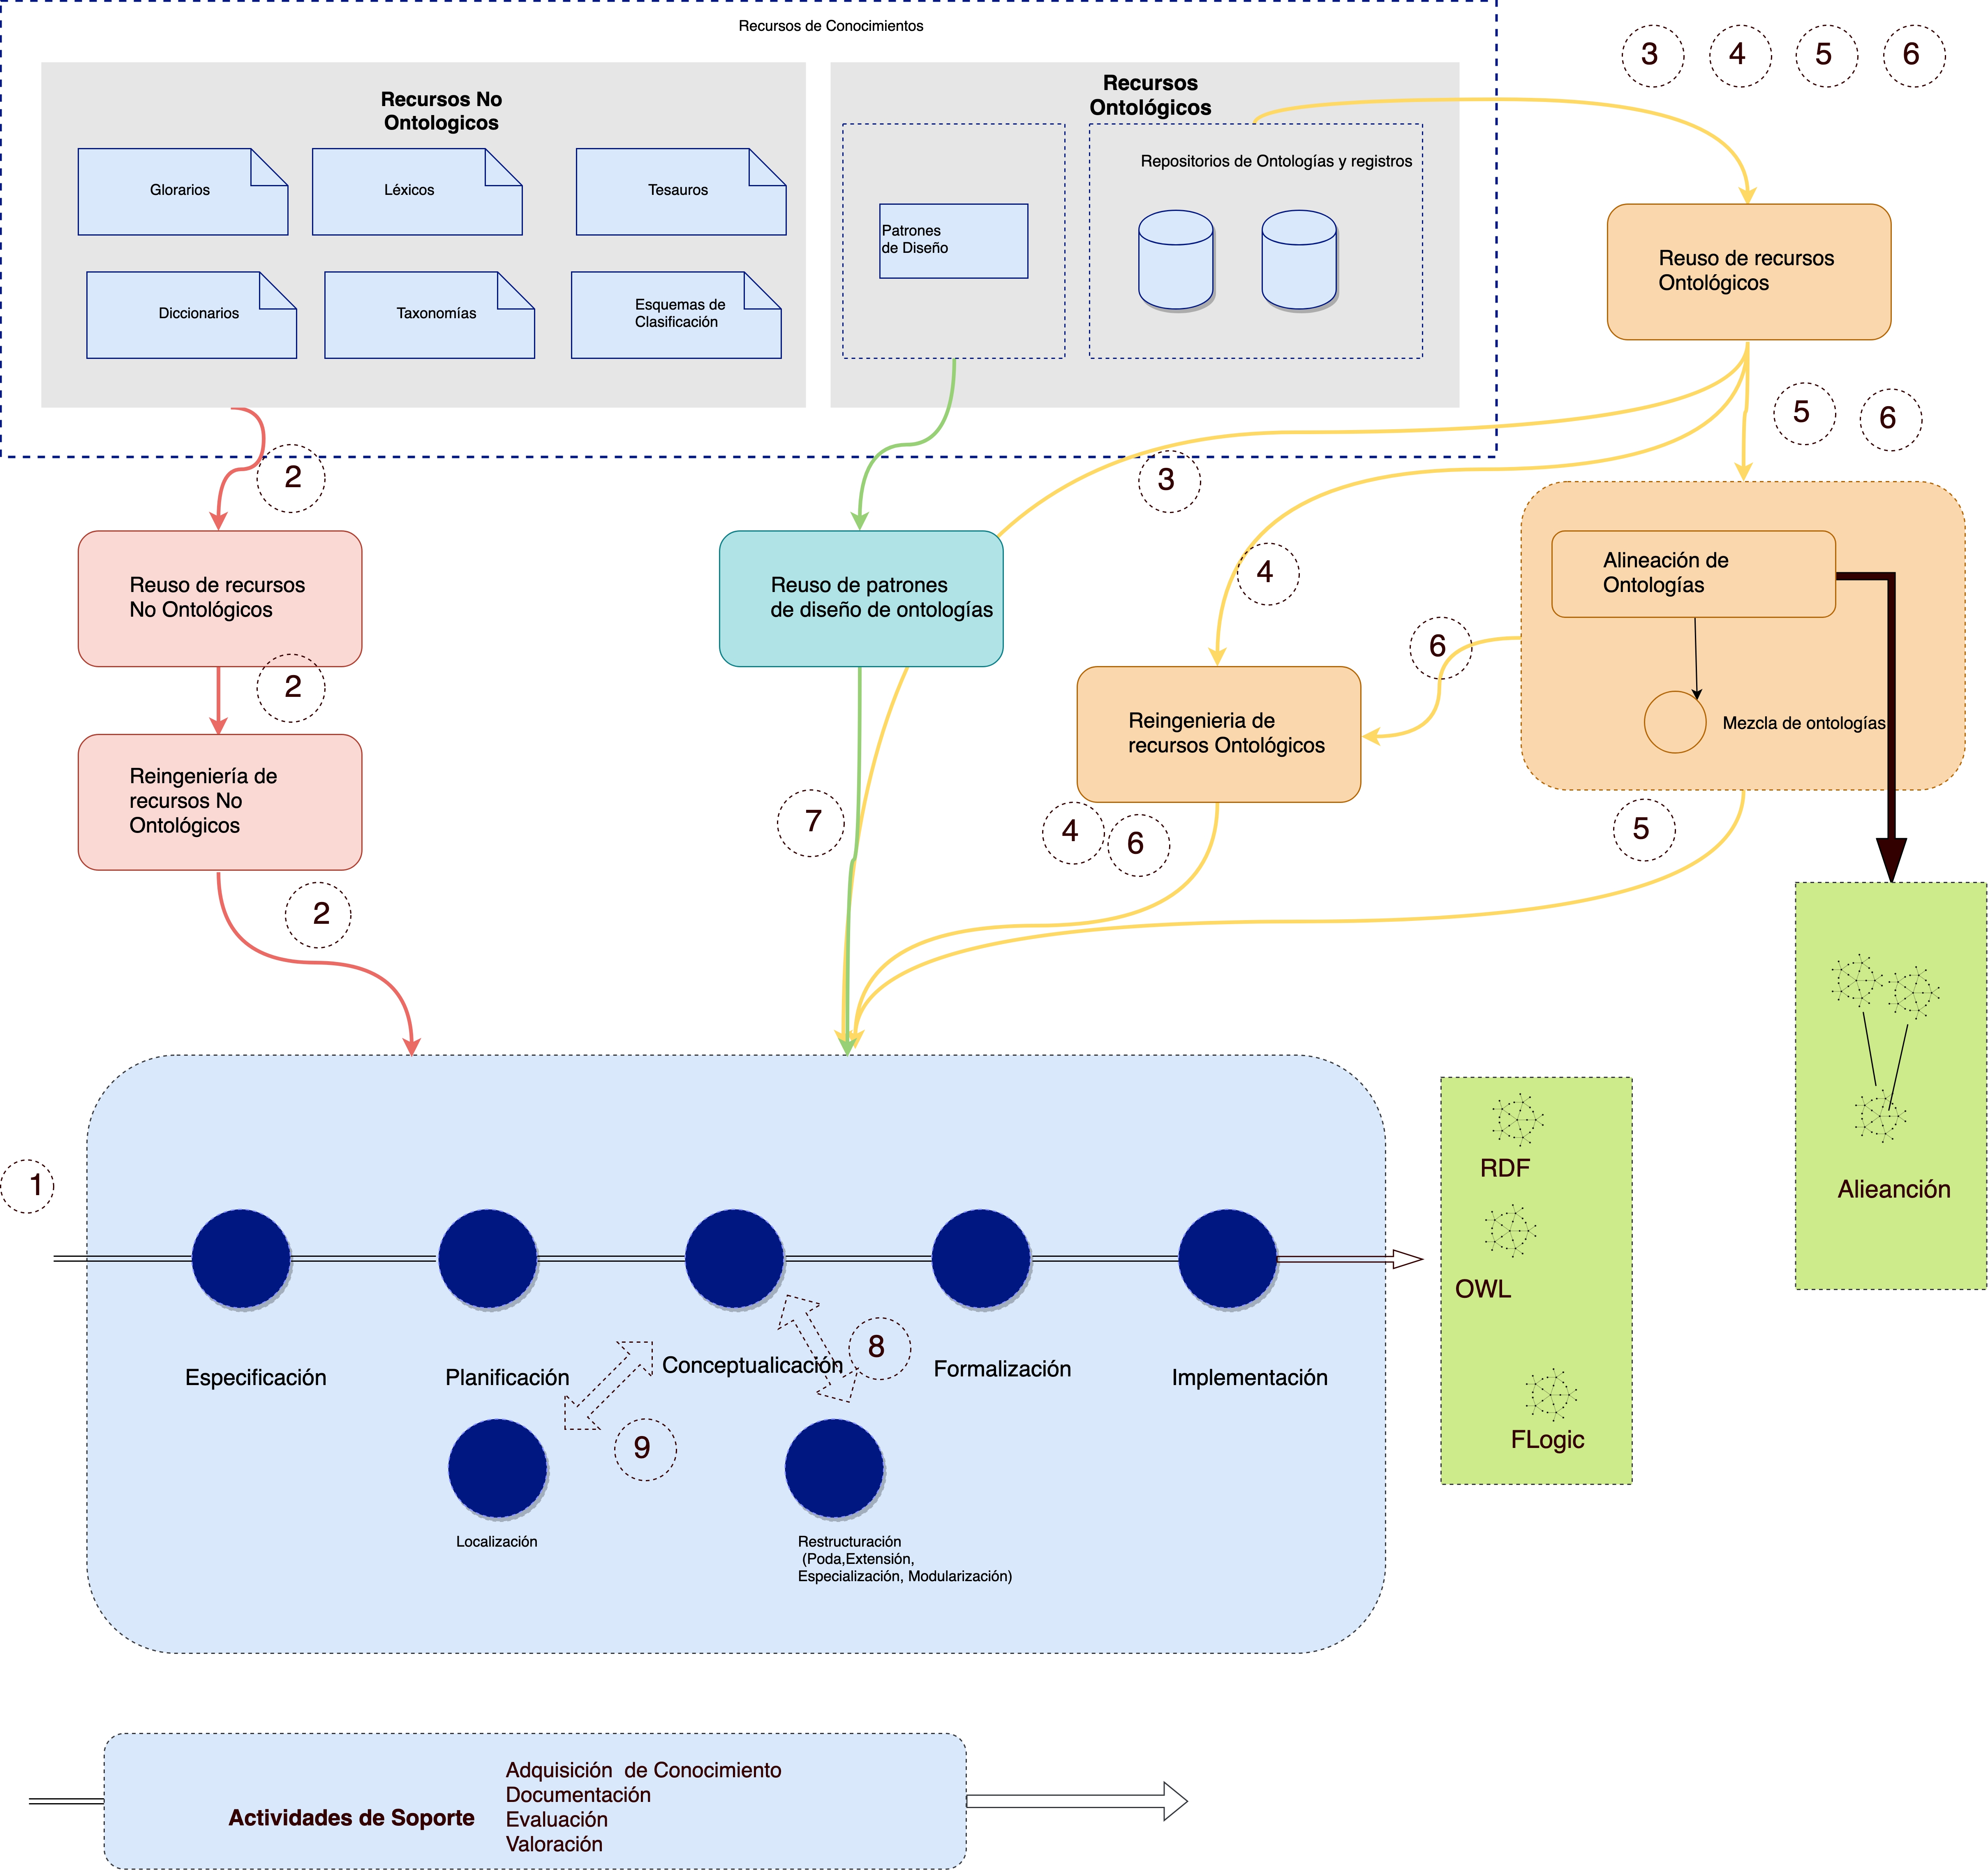
\includegraphics[width=150mm]{figuras/Diagramas-NeonProcess}
    \caption{Ciclo de vida de NeOn}
    \label{img:neon ciclo de vida}
    \end{figure}

El proceso de desarrollo de una ontología es definido como un proceso en el cual las necesidades de un usuario son convertidas a una ontología. Esto significa que el proceso se puede ver como un caso específico del proceso de desarrollo de software.	
El ciclo de vida es un modelo que describe cómo construir y mantener un proyecto ontológico, osea cómo ordenar los procesos y actividades en fases. Se pueden tener dos tipos de ciclo de vida que son:

\begin{itemize}
    \item Modelo de ciclo de vida de tipo cascada: En este modelo cada fase debe ser culminada antes de avanzar a la siguiente, no se permite retroceso excepto en el caso de la fase de mantenimiento. Este modelo es ideal cuando el tiempo de desarrollo es acotado y el dominio de conocimiento a modelar es bien conocido.
    \item Modelo de ciclo de vida de tipo iterativo-incremental: cada iteración es similar al modelo de cascada. Es ideal cual existe mucha incertidumbre acerca del alcance de la ontología a modelar.
\end{itemize}

A continuación exponemos los 5 modelos de ciclo de vida:	

\begin{description}
    \item[Modelo cascada de 4 fases.] Representa las etapas de una red de ontologías, comenzando con la Fase de Iniciación y yendo a través de la Fase de Diseño y Fase de Implementación hasta la Fase de Mantenimiento.
    \item[Modelo cascada de 5 fases.] Extiende el modelo de 4 fases con el reuso de recursos  ontológicos tales como son.
    \item[Modelo cascada de 5 fases + mezcla.] Es un caso especial del modelo de 5 fases. Incluye la Fase de Mezcla para obtener un nuevo recurso ontológico a partir de dos o más recursos ontológicos previamente seleccionados en la Fase de Reuso.
    \item[Modelo cascada de 6 fases.] Extiende el modelo de 5 fases con la Fase de Reingeniería. Permite la reingeniería de recursos de conocimiento (ontológicos y no-ontológicos). Puede ocurrir que algunos recursos de conocimiento son transformados en ontologías en la Fase de Reingeniería.
    \item[Modelo cascada de 6 fases + Mezcla.] Extiende el modelo de 6 fases incluyendo la Fase de Mezcla luego de la Fase de Reuso.
\end{description}

Los escenarios están ligados a un modelo dentro del ciclo de vida, como se muestra en la Tabla \ref{escenarios vs modelo}.

\begin{table}[tbp]
\centering
\caption{Escenarios vs Modelo}
\label{escenarios vs modelo}
\resizebox{15cm}{!} {
\begin{tabular}{|l|c|c|c|c|c|}
\hline
 & \multicolumn{1}{m{2cm}|}{Modelo de 4-fases} & \multicolumn{1}{m{2cm}}{Modelo de 5-fases} & \multicolumn{1}{|m{2cm}|}{Modelo de 5-fases + mezcla} & \multicolumn{1}{m{2cm}}{Modelo de 6-fases} & \multicolumn{1}{|m{2cm}|}{Modelo de 6-fases + mezcla} \\ \hline
 Escenario 1 & x & & & & \\ \hline
 Escenario 2 & & & & x & \\ \hline
 Escenario 3 & & x & & & \\ \hline
 Escenario 4 & & & & x & \\ \hline
 Escenario 5 & & & x & & \\ \hline
 Escenario 6 & & & & & x \\ \hline
 Escenario 7 & & & & x & \\ \hline
 Escenario 8 & & & x & & \\ \hline
 Escenario 9 & & & x & & \\ \hline
\end{tabular}
}
\end{table}

Cabe mencionar que estos escenarios se pueden combinar de maneras diferentes y flexibles, y que cualquier combinación de escenarios debería incluir el Escenario 1 porque este escenario está compuesto por las actividades centrales que deben realizarse en cualquier desarrollo de ontología.
En la Tabla \ref{tab:comparacion} se presenta un cuadro comparativo con las metodologías introducida en las secciones anteriores. 

\begin{table}[tbp]
\centering
\caption{Comparación de Metodologías de Desarrollo de Ontologías}
\label{tab:comparacion}
\resizebox{15cm}{!} {
\begin{tabular}{|l|l|l|l|l|}
\hline
\multicolumn{1}{|m{3cm}|}{Metodología/ Criterios} & \multicolumn{1}{m{3cm}}{Ontology Development 101} & \multicolumn{1}{|m{3cm}|}{OntoKnowledge} & \multicolumn{1}{m{3cm}}{Methontology} & \multicolumn{1}{|m{3cm}|}{NeOn Methodology} \\ \hline
\multicolumn{1}{|m{3cm}|}{Colaboración} & \multicolumn{1}{m{3cm}}{No} & \multicolumn{1}{|m{3cm}|}{No} & \multicolumn{1}{m{3cm}}{No} & \multicolumn{1}{|m{3cm}|}{Si} \\ \hline
\multicolumn{1}{|m{3cm}|}{Especificación} & \multicolumn{1}{m{3cm}}{Solo Preguntas de competencias} & \multicolumn{1}{|m{3cm}|}{Explícito} & \multicolumn{1}{m{3cm}}{Solo Preguntas de competencias} & \multicolumn{1}{|m{3cm}|}{Explícito} \\ \hline
\multicolumn{1}{|m{3cm}|}{Planeamiento} & \multicolumn{1}{m{3cm}}{No} & \multicolumn{1}{|m{3cm}|}{No} & \multicolumn{1}{m{3cm}}{No proveído} & \multicolumn{1}{|m{3cm}|}{Proveído} \\ \hline
\multicolumn{1}{|m{3cm}|}{Reuso de recursos ontológicos} & \multicolumn{1}{m{3cm}}{No proveído, solo algunos delineamientos} & \multicolumn{1}{|m{3cm}|}{No proveído, solo algunos delineamientos} & \multicolumn{1}{m{3cm}}{No proveído, solo algunos delineamientos} & \multicolumn{1}{|m{3cm}|}{Proveído} \\ \hline
\multicolumn{1}{|m{3cm}|}{Detalles de la Metodología} & \multicolumn{1}{m{3cm}}{Pocos Detalles} & \multicolumn{1}{|m{3cm}|}{Algunos detalles} & \multicolumn{1}{m{3cm}}{Algunos detalles} & \multicolumn{1}{|m{3cm}|}{Muchos detalles} \\ \hline
\multicolumn{1}{|m{3cm}|}{Dependiente de aplicación} & \multicolumn{1}{m{3cm}}{Independiente} & \multicolumn{1}{|m{3cm}|}{Independiente} & \multicolumn{1}{m{3cm}}{Independiente} & \multicolumn{1}{|m{3cm}|}{Independiente} \\ \hline
\multicolumn{1}{|m{3cm}|}{Audiencia} & \multicolumn{1}{m{3cm}}{Estudiantes y practicantes de ontologías} & \multicolumn{1}{|m{3cm}|}{Ingenieros en Ontologías} & \multicolumn{1}{m{3cm}}{Ingenieros en Ontologías e investigadores} & \multicolumn{1}{|m{3cm}|}{Ingenieros en sistemas, Ontologías y público en general} \\ \hline

\end{tabular}
}
\end{table}

En la Tabla \ref{tab:comparacion} cabe destacar que las 4 metodologías son las más populares dentro del desarrollo de las ontologías. En cuanto a la madurez y completitud de cada una podemos decir que la metodología NeOn es la más completa y madura, ya que la misma está basada en metodologías de desarrollo de software y metodologías de ingeniería de conocimiento.